\documentclass[12pt]{article}
\usepackage{amsmath,latexsym,amsfonts,amssymb,graphicx,amsthm,epsfig,enumerate}
\usepackage{tikz,verbatim} % adds charting fuctions

\linespread{1.2}

%\pagestyle{empty}

\begin{document}
		\title{Title} %add title here
		\author{Name} %add names here
		% add other necessary information here
		
		\maketitle
		\thispagestyle{empty}
		\newpage
		
		\section{Introduction}
		
		\subsection{Architecture}
		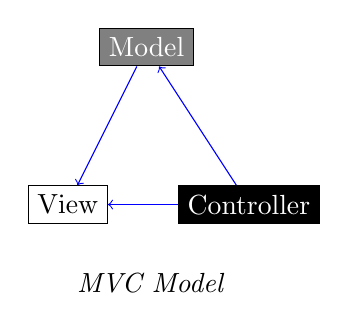
\begin{tikzpicture}
		% MVC Architecture
		\node[draw] (View) at (0,0) {View};
		\node[draw,fill=black,text=white] (Controller) at (2.3,0) {Controller};
		\node[draw,fill=gray,text=white] (Model) at (1,2) {Model};

		\draw[->,draw=blue] (Model) to (View);
		\draw[->,draw=blue] (Controller) to (View);
		\draw[->,draw=blue] (Controller) to (Model);
		\node at (1.0, -1.0) {\textit{ MVC Model}};
		
		\end{tikzpicture}
		\subsection{Technologies}
		
		\section{Modular Decomposition}
		
		\section{Module Guide}
		
		\section{Traceability}
		
		\section{Uses Relation}
		
		\section{Discussion}
		
		\subsection{Anticipated Changes}
		
		
	
\end{document}